% Thermostat Equation Annotation Diagram
% Maps trajectory distribution equation to thermostat example
% Annotations alternate above/below for clarity

\documentclass{article}
\usepackage[margin=0.2cm, paperwidth=19cm, paperheight=7cm]{geometry}
\usepackage{amsmath,amssymb}
\usepackage{tikz}
\usetikzlibrary{positioning, arrows.meta, calc}
\usepackage{xcolor}
\pagestyle{empty}

\definecolor{annotblue}{HTML}{4A90D9}
\definecolor{arrowgray}{HTML}{7F8C8D}

\begin{document}
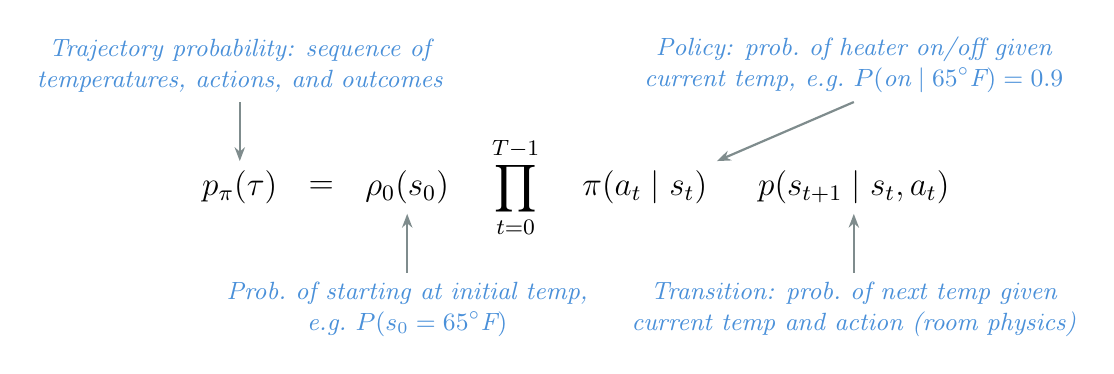
\begin{tikzpicture}[
    annot/.style={font=\small\itshape, text=annotblue, align=center},
    arrw/.style={-{Stealth[length=5pt]}, arrowgray, thick}
]

% Place each equation term as a separate node for precise arrow targeting
\node[font=\large] (lhs) at (0,0) {$p_{\pi}(\tau)$};
\node[font=\large, right=0.15cm of lhs] (eq) {$=$};
\node[font=\large, right=0.15cm of eq] (rho) {$\rho_0(s_0)$};
\node[font=\large, right=0.3cm of rho] (prod) {$\displaystyle\prod_{t=0}^{T-1}$};
\node[font=\large, right=0.3cm of prod] (policy) {$\pi(a_t \mid s_t)$};
\node[font=\large, right=0.4cm of policy] (trans) {$p(s_{t+1} \mid s_t, a_t)$};

% Annotations above: trajectory (term 1) and policy (term 3)
\node[annot, above=0.75cm of lhs] (tau-text) {
    Trajectory probability: sequence of\\
    temperatures, actions, and outcomes
};
\draw[arrw] (tau-text.south) -- (lhs.north);

\node[annot, above=0.75cm of trans] (pi-text) {
    Policy: prob.\ of heater on/off given\\
    current temp, e.g.\ $P(\text{on} \mid 65^\circ\text{F}) = 0.9$
};
\draw[arrw] (pi-text.south) -- (policy.north east);

% Annotations below: initial state (term 2) and transition (term 4)
\node[annot, below=0.75cm of rho] (rho-text) {
    Prob.\ of starting at initial temp,\\
    e.g.\ $P(s_0 = 65^\circ\text{F})$
};
\draw[arrw] (rho-text.north) -- (rho.south);

\node[annot, below=0.75cm of trans] (trans-text) {
    Transition: prob.\ of next temp given\\
    current temp and action (room physics)
};
\draw[arrw] (trans-text.north) -- (trans.south);

\end{tikzpicture}
\end{document}
